% RQ4
\section{Interpretability of tools}
\label{sec:interpretabilityoftools}
The prediction of performance of error detection tools gives another research direction, namely the dissection of this prediction.
Based on section \ref{sec:performanceprediction} and \ref{sec:toolranking}, with a set of input features and output values in the two tasks, the regression models can be analyzed to "explain" the inner workings of tools. Using feature importance identification methods depending on the specific regressor or general importance methods, the "weight" of a certain feature of the data profile can be translated to the performance of a certain tool with a specific configuration. The importance of features for each strategy can than be analyzed, to see if they correspond with the underlying techniques in these methods. If there are matches and mismatches, try to find why the misalignment occurs and see if improvements can be suggested for the error detection tools. A visual representation of making the error detection models interpretable, is shown in figure \ref{fig:method_interpret}.

\begin{figure}
    \centering
    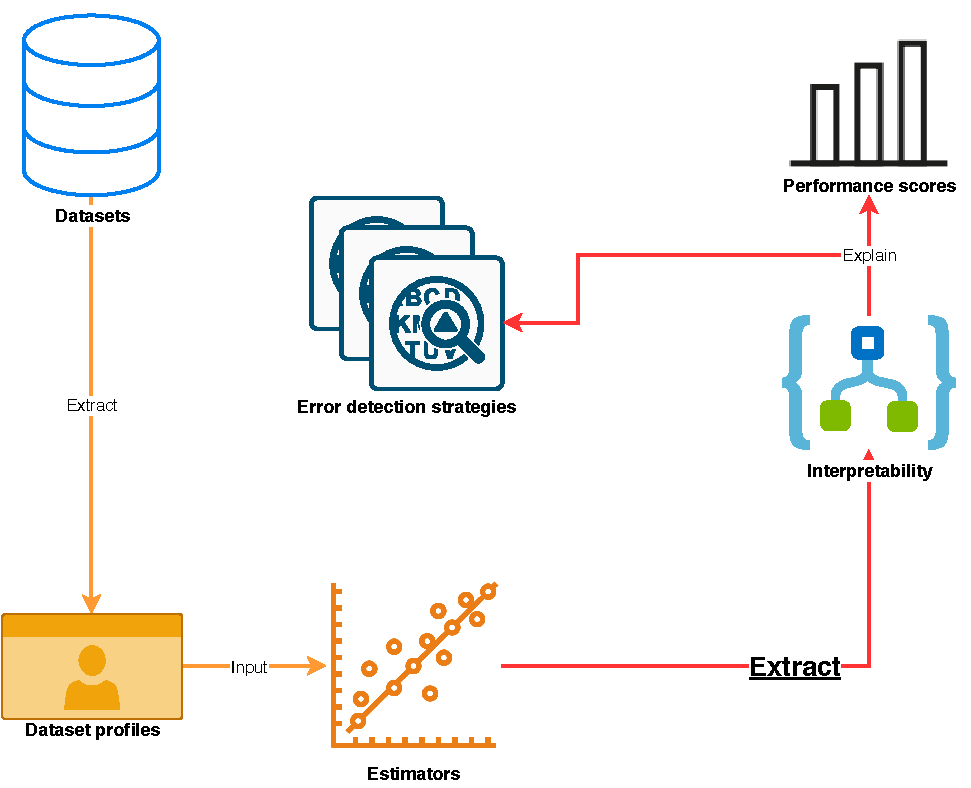
\includegraphics[width=0.9\textwidth]{thesis/Figures/Method/PerformanceEstimation-Interpretability.pdf}
    \caption{Adding interpretability into the flow of error detection}
    \label{fig:method_interpret}
\end{figure}

\subsection{Feature selection}
\label{subsec:featureselection}
Besides the learnable feature selection that will be used in the performance estimate pipeline of section \ref{sec:performanceprediction}, feature selection can also be done at the end of the estimation loop. Upon finding the most important features from the following section, a reduction of the dimensionality of the input to the estimator can be done, in order to improve the machine learning models, due to the curse of dimensionality otherwise. 

\subsection{Feature importance}
% According to the regression models
% Used as a proxy, something that is easy and quick to measure
Finding which data profile features are important for the regression model to estimate its performance, give insights to how a certain error detection strategy behaves. 

% Per tool
Permutation Importance

SHAP